\documentclass{../lista}

\begin{document}
	\cabecalho{1}{\red{Gabarito}}{Terra, Lua e Sol}{Iago Braz Mendes}

	\begin{questao}{1 ponto}
		Os primeiros eclipses foram registados há cerca de 4 mil anos na Babilônia. Ao longo da história, eles provocaram medo e admiração. Ao observarem os eclipses, povos de diferentes épocas relacionaram esse fenômeno à intervenção de figuras mitológicas que tentariam devorar os astros e a sua luz.

		\begin{pergunta}{0,5 ponto}
			Analise as 2 astrofotos abaixo -- tiradas pelo autor desta lista :) -- e marque o item que mostra um eclipse.
			\begin{multicols}{2}
				\begin{figure}[H]
					\centering
					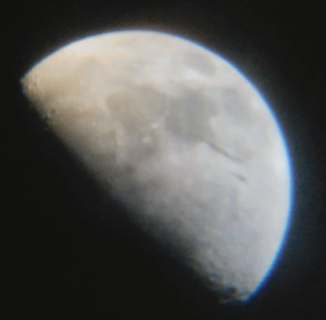
\includegraphics[width=.6\linewidth]{img/1a.png}
					\captionsetup{labelformat=empty}
					\caption{(a)}
					\end{figure}
				\begin{figure}[H]
					\centering
					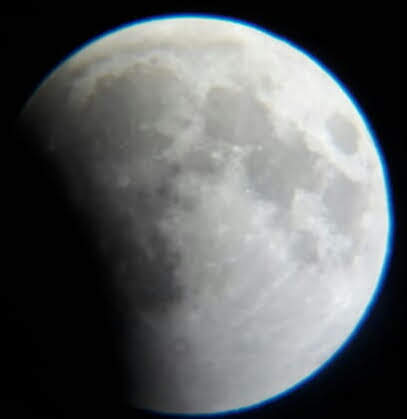
\includegraphics[width=.6\linewidth]{img/1b.jpg}
					\captionsetup{labelformat=empty}
					\caption{\red{(b)}}
				\end{figure}
			\end{multicols}

			\red{Perceba que, no item b, a parte escura está com um formato arredondado, o que só ocorre em eclipses. Inclusive, foi assim que, há muito tempo, Aristóteles sugeriu que a Terra devia ser redonda devido a sua sombra projetada na Lua.}
		\end{pergunta}

		\begin{pergunta}{0.25 ponto}
			Que tipo de eclipse é mostrado?
			\begin{alternativas}
				\alternativaMarcada Eclipse lunar
				\item Eclipse solar
			\end{alternativas}

			\red{A sombra da Terra está sendo projetada na Lua, então é um eclipse lunar. Só seria um eclipse solar caso a sombra do Sol estivesse sendo projetada na Terra.}
		\end{pergunta}
		
		\begin{pergunta}{0.25 ponto}
			Em qual fase lunar esse eclipse aconteceu?
			\begin{alternativas}
				\item Lua Nova
				\item Lua Crescente
				\alternativaMarcada Lua Cheia
				\item Lua Minguante
			\end{alternativas}

			\red{Eclipses lunares só podem ocorrer quando está Cheia, pois é preciso o alinhamento Sol-Terra-Lua. De modo análogo, eclipses solares só acontecem na Lua Nova, quando o alinhamento é Sol-Lua-Terra.}
		\end{pergunta}
	\end{questao}

	\begin{questao}{1 ponto}
		Analise, mais uma vez, a imagem do item que você \textbf{não} marcou como sendo um eclipse na questão anterior. Ela foi tirada no Hemisfério Sul por meio de um telescópio refletor. A imagem está exatamente como é observada na lente ocular, a qual produz uma imagem invertida.

		\begin{pergunta}{1 ponto}
			Levando em consideração o que foi dito, em qual fase lunar essa foto foi tirada?
			\begin{alternativas}
				\item Lua Nova
				\alternativaMarcada Lua Crescente
				\item Lua Cheia
				\item Lua Minguante
			\end{alternativas}

			\red{Como a imagem está invertida, a face iluminada é a oeste (no hemisfério sul, o lado esquerdo). Dessa forma, podemos afirmar que a foto foi tirada na Lua Crescente. Se a face iluminada fosse a leste, a Lua seria Minguante.}
		\end{pergunta}
	\end{questao}

	\begin{questao}{1 ponto}
		1 ano terrestre é comumente relacionado ao intervalo de tempo correspondente à translação completa da Terra em torno do Sol. Contudo, o valor exato de 1 ano varia de acordo com o método de análise. Nesse sentido, temos duas definições principais para essa medida de tempo: Ano Tropical e Ano Sideral.
		
		\begin{pergunta}{0,25 ponto}
			Qual o referencial na medida do Ano Tropical?
			\begin{alternativas}
				\item Movimento Retrógrado de Marte
				\alternativaMarcada Equinócio Vernal (início das estações do ano)
				\item Ápex (ponto para o qual o Sol se dirige)
				\item Periélio ou Afélio
			\end{alternativas}

			\red{O Ano Tropical é o intervalo de tempo entre duas passagens consecutivas do Sol pelo ponto Vernal -- ponto da Esfera Celeste onde se encontra o Sol no início das estações (equinócio de março).}
		\end{pergunta}
		
		\begin{pergunta}{0,25 ponto}
			Qual o referencial na medida do Ano Sideral?
			\begin{alternativas}
				\item Planetas do Sistema Solar
				\item Galáxia de Andrômeda
				\item Quasares
				\alternativaMarcada Estrelas de Fundo
			\end{alternativas}

			\red{O Ano Sideral é o intervalo de tempo entre duas passagens consecutivas do Sol pela mesma posição de acordo com as estrelas de fundo -- estrelas tão distantes que podem ser consideradas fixas na Esfera Celeste para distâncias pequenas como dentro do Sistema Solar.}
		\end{pergunta}
		
		\begin{pergunta}{0,25 ponto}
			O Ano Tropical tem duração de 365,2564 dias solares médios, enquanto o Ano Sideral possui 365,2422 dias solares médios. Qual é o \textbf{principal} movimento terrestre responsável por essa diferença?
			\begin{alternativas}
				\item Rotação da Terra
				\item Translação da Terra
				\alternativaMarcada Precessão dos Equinócios
				\item Nutação
			\end{alternativas}

			\red{A precessão dos equinócios é o movimento terrestre responsável por alterar a direção do eixo de rotação. Com isso, a relação entre as coordenadas celestes e eclípticas sofre pequenas alterações ao longo do seu período de 25.770 anos.}
		\end{pergunta}
		
		\begin{pergunta}{0,25 ponto}
			Geralmente, usamos 365,25 dias solares médios como uma aproximação para a duração do ano na Astronomia. Contudo, o nosso calendário possui 365 dias, o que deixa cerca de $\frac{1}{4}$ dia sobrando. Para consertar isso, temos o ano bissexto, o qual possui 366 dias solares médios e segue uma regra de 3 exigências. Pensando nisso, marque a seguir somente o(s) ano(s) que é(são) bissexto(s):
			\begin{alternativas}
				\alternativaMarcada 2400
				\item 1846
				\item 2100
				\alternativaMarcada 1960
			\end{alternativas}

			\red{Basta conferir as 3 exigências: 1) O ano deve ser múltiplo de 4; 2) O ano não pode ser múltiplo de 100; 3) A exigência 2 não vale, caso o ano seja múltiplo de 400.}
			\red
			{
				\begin{itemize}
					\item $2400$ é múltiplo de 4, de 100 e de 400. Portanto, é bissexto devido à exigência 3.
					\item $1846$ não é múltiplo de 4. Então, não é bissexto devido à exigência 1.
					\item $2100$ é múltiplo de 4 e de 100, e não é múltiplo de 400. Então, não é bissexto devido à exigência 2.
					\item $1960$ é múltiplo de 4. Então, é bissexto devido à exigência 1.
				\end{itemize}
			}
		\end{pergunta}
	\end{questao}

	\begin{questao}{1 ponto}
		Loinha -- uma estudante que usou muito o site da LOA -- foi medalhista de ouro na OBA e está atualmente estudando para as Seletivas. Em seus estudos, deparou-se com vários esquemas altazimutais e resolveu criar um com base no seu local de moradia. Assim, ela desenhou a seguinte representação:
		\begin{figure}[H]
			\centering
			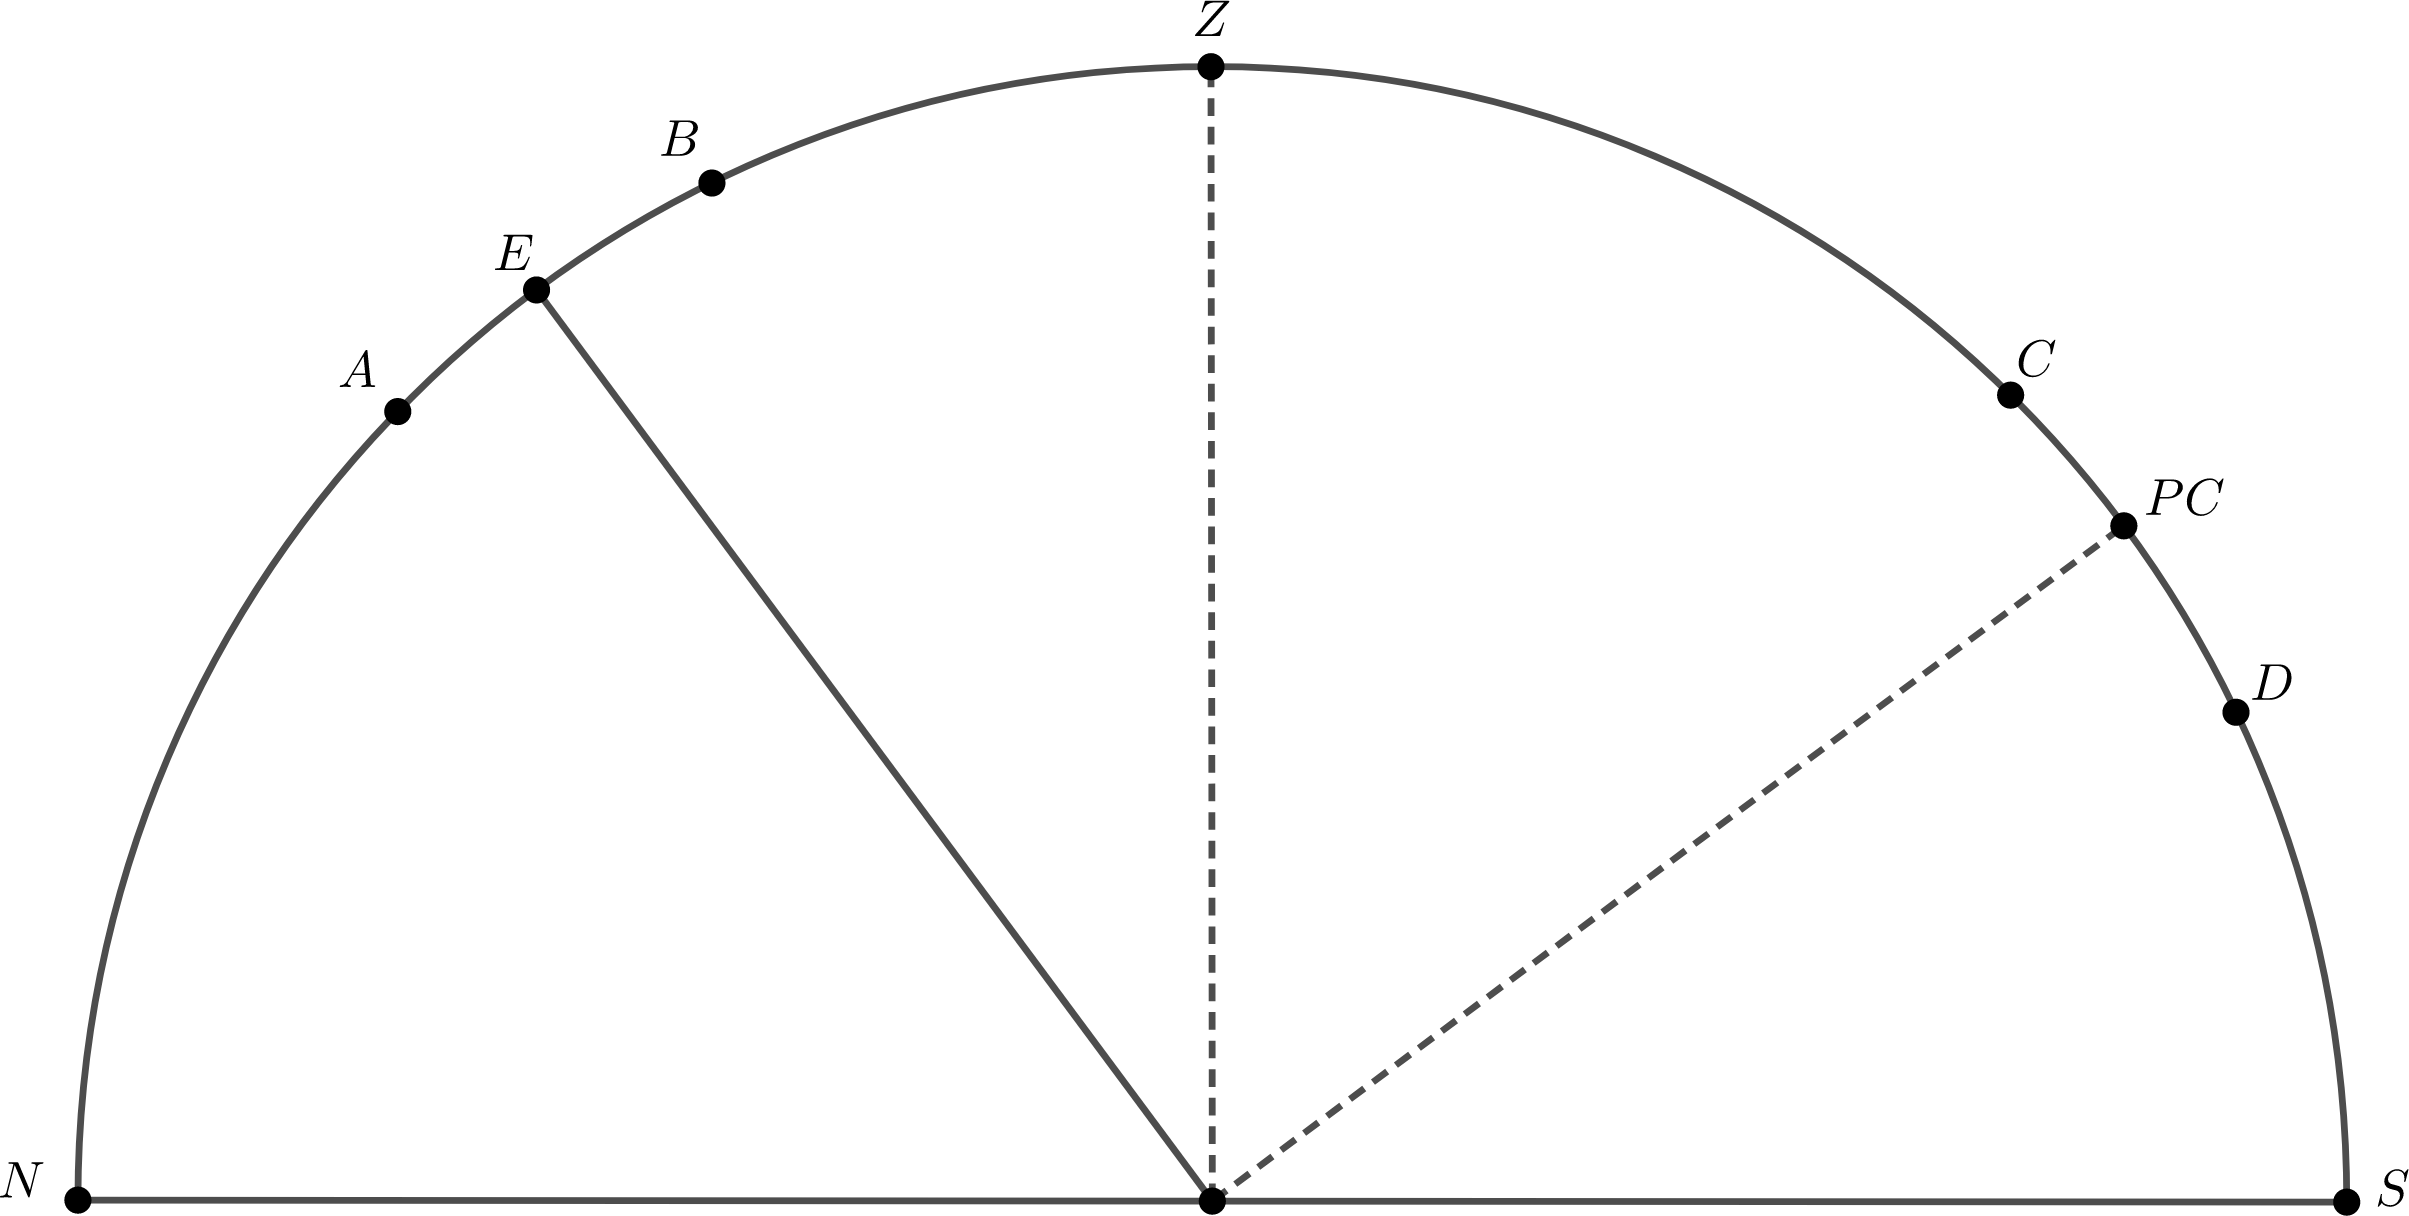
\includegraphics[scale=1.2]{./img/4.png}
		\end{figure}
		Nela, a linha horizontal representa o horizonte; o semiarco, a esfera celeste; $N$ e $S$, pontos cardeais norte e sul, respectivamente; $E$, o equador celeste (perceba que estamos olhando de lado, o que torna uma circunferência num segmento de reta); $PC$, o Polo Celeste elevado; $Z$, o zênite; e $A$, $B$, $C$ e $D$ pontos estratégicos na esfera celeste. \linebreak
		Como Loinha adora colocar em prática os conceitos aprendidos no site da LOA, fez alguns registros. Primeiramente, anotou a data e o horário: 22/06 (solstício de junho) ao meio-dia.\linebreak
		Observação: considere o mesmo horário para as perguntas.
		
		\begin{pergunta}{0,5 ponto}
			Depois, ele decidiu registrar em que posição o Sol se encontrava naquele momento. Qual a resposta correta?
			\begin{alternativas}
				\alternativaMarcada $A$
				\item $B$
				\item $C$
				\item $D$
			\end{alternativas}

			\red{No solstício de junho, o Sol está sobre o Trópico de Câncer, marcando o Verão no Hemisfério Norte e o Inverno no Hemisfério Sul. Portando, o Sol deve estar numa posição ao norte do Equador Celeste, o que só é verdade para $A$.}
		\end{pergunta}

		\begin{pergunta}{0,5 ponto}
			Animado para ver o comportamento das sombras, Loinha fincou uma haste na projeção do zênite no chão (centro da semicircunferência). Com a ajuda de uma bússola, anotou a direção cardeal para a qual a sombra apontava. Qual foi a anotação?
			\begin{alternativas}
				\item Norte
				\item Leste
				\alternativaMarcada Sul
				\item Oeste
			\end{alternativas}

			\red{Como o Sol está na direção Norte e no Meridiano Local (devido ao fato de ser meio-dia), a sombra deve apontar para a direção Sul.}
		\end{pergunta}
	\end{questao}

	\begin{questao}{1 ponto}
		Para as perguntas desta questão, considere o contexto da questão anterior.

		\begin{pergunta}{0,5 ponto}
			Em que lugar Loinha mora?
			\begin{alternativas}
				\item Hemisfério Norte
				\item Equador
				\alternativaMarcada Hemisfério Sul
			\end{alternativas}

			\red{O polo elevado está apontando para a direção Sul, o que só ocorre no Hemisfério Sul. No Hemisfério Norte, o polo elevado aponta para a direção Norte e, no Equador, não há polo elevado.}
		\end{pergunta}

		\begin{pergunta}{0,5 ponto}
			No momento dos registros, que solstício estava ocorrendo no Hesisfério Norte e Sul, respectivamente?
			\begin{alternativas}
				\item Solstício de Verão e Solstício de Verão
				\alternativaMarcada Solstício de Verão e Solstício de Inverno
				\item Solstício de Inverno e Solstício de Inverno
				\item Solstício de Inverno e Solstício de Verão
			\end{alternativas}

			\red{Como o Sol está sobre o Trópico de Câncer, a insolação no Hemisfério Norte será maior do que no Hemisfério Sul. Portando, será Solstício de Verão naquele e de Inverno neste.}
		\end{pergunta}
	\end{questao}

	\encerramento
\end{document}